\documentclass[a4paper,10pt]{article}
%\usepackage[utf8]{inputenc}
\usepackage[a4paper,margin=2cm]{geometry}
\usepackage[T1]{fontenc}
\usepackage[ansinew]{inputenc}
\usepackage{ae}
\usepackage{amsmath}
\usepackage{amsfonts}
\usepackage{amsthm}
\usepackage{amssymb}
\usepackage{array}
%\usepackage[dutch]{babel}
\usepackage[usenames,dvipsnames]{color}
\usepackage{enumitem}
\usepackage{epsfig}
\usepackage{float}
\usepackage{graphics}
\usepackage{listings}
\usepackage{makeidx}
\usepackage{parskip}
\usepackage[section]{placeins}
\usepackage{siunitx}
\usepackage{titling}
\usepackage{hyperref}
\usepackage{url}
\usepackage{natbib}



\newlist{SubItemList}{itemize}{1}
\setlist[SubItemList]{label={$-$}}

\let\OldItem\item
\newcommand{\SubItemStart}[1]{%
    \let\item\SubItemEnd
    \begin{SubItemList}[resume]%
        \OldItem #1%
}
\newcommand{\SubItemMiddle}[1]{%
    \OldItem #1%
}
\newcommand{\SubItemEnd}[1]{%
    \end{SubItemList}%
    \let\item\OldItem
    \item #1%
}
\newcommand*{\SubItem}[1]{%
    \let\SubItem\SubItemMiddle%
    \SubItemStart{#1}%
}%

\newcommand{\subtitle}[1]{%
  \posttitle{%
    \par\end{center}
    \begin{center}\large#1\end{center}
    \vskip0.5em}%
}


%opening
\title{Introduction}
\author{Tamar Huygen}


\begin{document}

\maketitle

\section*{General Introduction}


-climate change
-our solution
-modelling

\subsection{Sustainability (under construction)}\label{sec:sus}
The main returning theme in this paper is stability. The word stability has 
different meanings in different contexts. In this paper several definitions of 
stability will be discussed. We will start with one that has to do with one of 
the greatest challenges that mankind has to face in this time. The stability of 
our own population, humanity, on this planet.
We might think that we will always be able to live like we were used to on our 
planet, but considering our own population dynamics (see figure 
\ref{fig:owndyn}) and the accompanying demand for energy and food. We can safely 
assume that using resources we cannot replenish, will not be a stable strategy 
and sooner or later one of the irreplaceable resources will run out. When that 
happens we have to see whether the other resources are able to fill in the gap. 
Until that happens we have to look for more sustainable ways of producing food 
and energy. Resources that cannot run out fast, such as sunlight or geothermal 
energy, have the advantage that they will be a reliable energy source for as 
long as humanity lives on this planet.

In the way we are using the recourses of the planet now we also have multiple 
environmental issues. Pollution of the environment may give an (economic) 
advantage on the short term, but polluting strategies are certainly not feasible 
considering longer timespans. 
Then there is also the problem of global warming. Because of the increasing use 
of fossil fuels a lot more CO$_{2}$ is released in the atmosphere and CO$_{2}$ 
levels have been rising. Although there are gasses with higher global warming 
potential, a slight change in the balance of gases in the atmosphere, can have 
an effect on temperature. This slight effect can also have an effect on other 
sources of greenhouse gases, such as release of methane from permafrost tundras 
which are now thawing, enhancing the greenhouse effect. This gas-compositions 
shift and accompanying temperature shift will have major ecological and 
economical consequences on our planet. If we want to slow this process down it 
is of major importance that we reduce the emission of greenhouse gases and 
CO$_2$.

This is were the biobased economy comes in. More and more entrepreneurs and 
scientists are looking for less polluting ways to produce, where possible also 
with less CO$_2$ emission. They can do this with the help of biotechnological 
advances. In biotechnology, there are also still a lot of challenges. In the 
past food crops have been used to create fuel in a biobased manner. This caused 
the crop prices to rise in certain areas, which is seen as a great disadvantage. 
We have to find a way to produce in a sustainable manner, without competing with 
food. By choosing a non crop organism, which harvests light and CO$_2$, like 
Synechocystis, we might get a small step closer to reach this goal. 

In an ideal world we would have closed carbon cycles. That which we produce in 
CO$_2$ would also be consumed. In this way we would enhance the stability of the 
environment in which mankind seems to prevail. 

\begin{figure}[!ht]
 \begin{center}  
  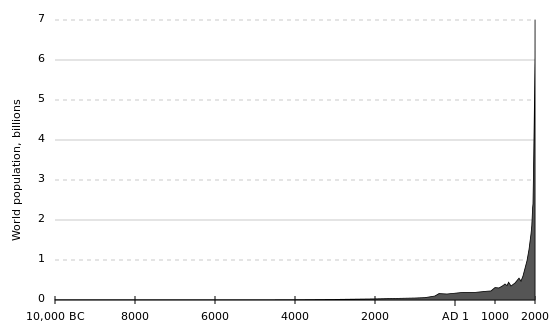
\includegraphics[width=8cm]{human_population_curve.png}
  \caption{Our own population dynamics so far.}
  \label{fig:owndyn}
 \end{center}
\end{figure}

\subsection{The search for a sustainable solution and synthetic biology}
A lot of different approaches in the search for sustainable production and 
energy harvest have been used. 

\subsection{The team iGEMAmsterdam 2015 Solution}
The iGEM team of 


\bibliographystyle{unsrtnat}
\bibliography{iGEMrefs}

\end{document}